\bookchapter{Chapitre 60 : Monter l’environnement de développement — Xcode et le premier projet}

\chapterintro{Pour bien faire le travail, il faut d’abord affûter ses outils. Dans ce chapitre, on monte la « cuisine » : installer Xcode, faire tourner le simulateur, créer le tout premier projet iOS de ta vie, puis décortiquer la structure du projet pour tout comprendre. Une fois l’environnement prêt, tu verras pour la première fois ton code se transformer en bouton cliquable — un instant que beaucoup gardent toute leur vie en mémoire.}

\booksection{S’équiper d’un Mac}

Commençons par le prérequis : le développement iOS doit se dérouler sur macOS. Sans Mac, trois options : en acheter un (un Mac mini ou un MacBook Air d’occasion suffit largement), louer un Mac dans le cloud pour une courte durée, ou commencer par lire la huitième partie, « Android en pratique » (possible sous Windows).

\begin{center}
\begin{tabularx}{\linewidth}{|X|X|X|}
\hline
\textbf{Élément de configuration} & \textbf{Minimum requis} & \textbf{Zone de confort (recommandé)} \tabularnewline
\hline
Puce & Apple Silicon (M1 ou plus) & M2 ou plus récent \tabularnewline
Mémoire & 8GB & 16GB \tabularnewline
Disque & Prévoir 40 Go et plus (Xcode est bien dodu) & 256 Go pour commencer \tabularnewline
Système & Le dernier macOS & Mises à jour automatiques maintenues \tabularnewline
\hline
\end{tabularx}
\end{center}

\begin{center}\small\color{gray}Configuration de référence d’un Mac de développement (août 2026)\end{center}

\begin{tcbinfo}{Astuce : sans Mac, tu peux déjà apprendre le langage}
Swift Playgrounds, gratuit sur iPad, permet d’apprendre les bases du langage Swift (sans Mac) ; il s’installe même sur iPhone. Familiarise-toi d’abord dans Playgrounds avec les notions de langage du chapitre 61, et tu décolleras dès que tu auras un Mac. Préparer ses outils ne fait jamais perdre de temps : c’est exactement ça.

\end{tcbinfo}

\booksection{Installer Xcode}

Xcode est l’environnement de développement intégré officiel d’Apple, et il est gratuit. Trois étapes suffisent :

\begin{enumerate}
  \item Sur Mac, ouvre l’App Store, cherche « Xcode » et clique sur Installer — attention, il pèse plusieurs Go, choisis un créneau avec du bon réseau ;
  \item au premier lancement après l’installation, accepte le contrat et laisse se terminer l’installation des composants (c’est automatique) ;
  \item dans le menu Xcode Settings Locations, vérifie que Command Line Tools est bien sélectionné — les outils en ligne de commande sont le préalable de beaucoup de scripts et d’outils tiers.
\end{enumerate}

\begin{tcbwarn}{Attention : le jeu d’appariement entre versions et système}
Un Xcode récent exige souvent le dernier macOS, et un vieux Mac reste coincé sur une version ancienne. Pour publier sur l’App Store, Apple demande une version assez récente de Xcode (avec en général un délai de grâce). Ne reporte donc pas trop les mises à jour du système — les développeurs iOS sont ceux qui courtisent le plus assidûment les nouveautés.

\end{tcbwarn}

\booksection{Créer ton premier projet}

Ouvre Xcode Create New Project choisis iOS le modèle App, puis remplis :

\begin{center}
\begin{tabularx}{\linewidth}{|X|X|X|}
\hline
\textbf{Élément} & \textbf{Quoi remplir} & \textbf{Explication} \tabularnewline
\hline
Product Name & MyFirstApp & Nom de l’app \tabularnewline
Team & Ton identifiant Apple (gratuit) & Pour la signature, un compte personnel suffit \tabularnewline
Organization Identifier & com.example & Se combine au Product Name pour former l’identifiant du bundle \tabularnewline
Interface & SwiftUI & Le framework fil conducteur de ce livre \tabularnewline
Language & Swift & Sans commentaire \tabularnewline
\hline
\end{tabularx}
\end{center}

\begin{center}\small\color{gray}Les cinq champs à remplir à la création du projet\end{center}

Après avoir cliqué sur Create, Xcode génère un projet qui tourne immédiatement. Choisis un simulateur en haut à gauche (par exemple iPhone 17) et clique sur > — quelques secondes plus tard, une fenêtre affichant « Hello, world! » apparaît sur l’écran du simulateur. Ta première app iOS vient de naître.

\booksection{Anatomie du projet : à quoi sert chaque fichier}

À gauche se trouve le navigateur de projet ; en tant que débutant, il te suffit de reconnaître ceci :

\begin{center}
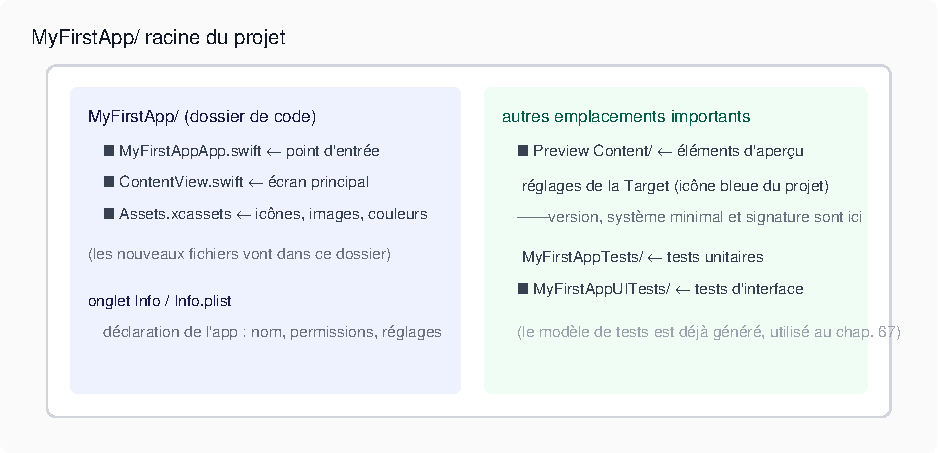
\includegraphics[width=0.92\linewidth]{figures/fig-di-liu-shi-zhang-1}
\\[2pt]\small Figure 2 : la structure d’un projet Xcode que tout débutant doit connaître
\end{center}

\begin{itemize}
  \item MyFirstAppApp.swift : le point d’entrée du programme ; en SwiftUI, il ne compte que quelques lignes — « démarre, puis affiche l’écran principal » ;
  \item ContentView.swift : la vue de l’écran principal ; tout ce que tu vois en ce moment est ici ;
  \item Assets.xcassets : l’entrepôt des ressources — icônes, images et couleurs se rangent ici ;
  \item Réglages du Target : clique sur l’icône bleue du projet à gauche pour y entrer ; le numéro de version, la version minimale d’iOS et la signature s’y trouvent. Le nom d’affichage de l’app et l’icône se règlent aussi ici.
\end{itemize}

\booksection{Débogage sur appareil réel : installer l’app dans ton iPhone}

\booksection{Astuces d’efficacité dans Xcode : les cinq « raccourcis bonus » du débutant}

Une fois rodés, ces raccourcis te donneront des allures de « grand pro » :

\begin{center}
\begin{tabularx}{\linewidth}{|X|X|X|}
\hline
\textbf{Action} & \textbf{Raccourci} & \textbf{Effet} \tabularnewline
\hline
Exécuter & CmdR & Compiler et lancer \tabularnewline
Ouvrir/basculer l’aperçu du canevas & OptionCmd & L’interrupteur du WYSIWYG \tabularnewline
Formater l’indentation & CtrlI & Réajuster automatiquement l’indentation du code sélectionné \tabularnewline
Ouvrir un fichier à la volée & CmdO & Tape le nom du fichier, il s’ouvre à la seconde (le plus utilisé !) \tabularnewline
Commenter/décommenter & Cmd/ & Activer/désactiver du code à la volée pendant le débogage \tabularnewline
\hline
\end{tabularx}
\end{center}

\begin{center}\small\color{gray}Raccourcis très utilisés de Xcode (le kit de cinq du débutant)\end{center}

Deux bonus cachés : le multi-simulateur (faire tourner en même temps iPhone et iPad pour comparer les dispositions) et la bibliothèque d’extraits de code (glisse tes quelques lignes favorites dans le panneau Snippets à droite, et insère-les en un clic la prochaine fois) — utilise ces outils d’efficacité, et le tour de main viendra tout seul.

\booksection{Débogage sur appareil réel : installer l’app dans ton iPhone}

Le simulateur est bien, mais l’appareil réel reste la destination finale. Avec un identifiant Apple gratuit, tu peux déboguer sur un vrai appareil :

\begin{enumerate}
  \item relie l’iPhone par câble (ou débogue en sans fil sur le même Wi-Fi) ;
  \item dans la liste des appareils en haut de Xcode, choisis ton téléphone ; au premier essai, il te proposera de te connecter à ton identifiant Apple et configurera la signature automatiquement ;
  \item sur l’iPhone, [Réglages] [Général] [VPN et gestion des appareils] accorde ta confiance au certificat de développeur ;
  \item clique sur >, et l’app s’installe dans l’appareil réel.
\end{enumerate}

\begin{tcbwarn}{Attention : la « limite de sept jours » du compte gratuit}
Une app signée avec un identifiant Apple gratuit expire au bout de 7 jours (il suffit de relancer une fois pour la renouveler). C’est un mécanisme anti-abus d’Apple, largement suffisant pour la phase d’apprentissage ; le compte développeur payant (99 dollars par an) n’a pas cette limite, le détail au chapitre 67.

\end{tcbwarn}

\booksection{Premier essai + premiers secours contre les erreurs courantes}

\booksection{Premier essai + premiers secours contre les erreurs courantes}

Ouvre ContentView.swift, remplace le texte de Text(“Hello, world!”) par ton prénom, puis relance avec CmdR — quelques secondes plus tard, ton prénom s’affiche sur le simulateur. Félicitations, tu viens d’accomplir ta première boucle complète « modifier le code compiler installer exécuter ».

\begin{center}
\begin{tabularx}{\linewidth}{|X|X|X|}
\hline
\textbf{Symptôme d’erreur} & \textbf{Cause fréquente} & \textbf{Remède} \tabularnewline
\hline
Erreur de signature (Signing) & Team non sélectionnée, certificat expiré & Dans Target Signing, coche ton compte ; avec un compte gratuit, relance une fois \tabularnewline
Simulateur en écran noir / impossible à ouvrir & Image corrompue & Menu Device Erase All Content ; ou supprime le simulateur et recrée-le \tabularnewline
Téléchargement de Xcode trop lent / installation impossible & Le réseau de l’App Store s’affole & Change de créneau ; ou télécharge le paquet .xip hors ligne depuis le site des développeurs Apple \tabularnewline
\hline
\end{tabularx}
\end{center}

\begin{center}\small\color{gray}Table de premiers secours contre les erreurs d’environnement du débutant\end{center}

\begin{tcbpractice}{À toi de jouer : achève ta liste des « rituels du développeur »}
(1) Installe Xcode et fais tourner le simulateur ; (2) lance une fois ton app sur un appareil réel et garde une capture en souvenir ; (3) remplace le texte Hello par ton prénom ; (4) dans les réglages du Target, change le nom d’affichage de l’app en « Ma première app ». Ces quatre étapes faites, tu es quelqu’un qui possède une création.

\end{tcbpractice}

\begin{tcbsummary}{Résumé du chapitre}
\begin{itemize}
  \item Prérequis dur : Mac + Xcode ; sans Mac, commence par apprendre le langage avec Swift Playgrounds sur iPad
  \item Xcode s’installe depuis l’App Store ; une version neuve exige un système à jour, ne tarde pas à mettre à jour
  \item Les cinq éléments d’un nouveau projet : nom, Team, identifiant d’organisation, SwiftUI, Swift
  \item La maxime du projet : tout le code est dans le dossier MyFirstApp/ ; les réglages du Target gèrent version et signature
  \item Avec un identifiant Apple gratuit, la signature sur appareil réel est limitée à 7 jours ; le compte payant n’a pas cette limite
  \item Le quotidien du développeur = modifier le code CmdR observer le résultat, encore et encore
\end{itemize}

\end{tcbsummary}
